\chapter{Predicting Legislative Votes with Text Models}
\label{chapter:predicting_votes}

In the United States, as in many Western democracies, laws are made by
committees of lawmakers.  A defining characteristic of these
committees is that each member casts a vote indicating whether she
supports or rejects the proposed legislation. Legislative behavior
centers around these votes, and it is a common goal of quantitative
political science to characterize patterns of lawmakers' behavior with
these votes. Voting behavior exhibits enough of a regularity that
simple statistical models easily capture the broad political structure
of legislative bodies.

One of these models is the \emph{ideal point model}, a mainstay in
quantitative political science for analyzing
votes~\citep{clinton:2004}.  It posits a latent ``political space''
along the real line and assumes each lawmaker has a position in that
space; bills take a position in a related latent space (look ahead to
\myfig{example_ideal_points} for an intuition of these positions).
%% The legislator's position is
%% called an \textit{ideal point} because it represents the state of the
%% world that maximizes her utility. The model assumes that whether a
%% legislator votes \verb!yea! on a bill depends on parameters of that
%% bill that describe how close it moves the world to her ideal
%% point.\footnote{These assumptions stem from a particular utility
%%   model, and this methodology is an instance of the
%%   \textit{item-response} model from psychometrics and educational
%%   testing \cite{lord:1980}.  Each bill also has another variable, the
%%   \textit{difficulty}, which is described below but omitted in the
%% introduction.}
A lawmaker's probability of voting \verb!Yea! on pending legislation
is then characterized by her position on this real line and parameters
specific to that legislation.

Just as we saw with the last chapter's spatial models, ideal point
models can be used to interpret lawmakers' positions on the political
spectrum and to represent votes meaningfully.\footnote{The
  interpretation of a lawmaker's latent position and a bill's position
  in the same space are slightly more nuanced than the last chapter.
  We clarify this relationship in the next section.}  However, ideal
point models have certain limitations.  One important limitation of
these models is that they are not \emph{predictive} models: while they
can be used to model the bills that have been voted on, they cannot be
used to predict lawmakers' votes on new bills.  (A second limitation
of these models is that lawmakers do not fit neatly into the
assumptions made by such models.  We address this limitation in the
next chapter.)  In this chapter we will extend the ideal point model
so that we can make predictions about how lawmakers will vote on bills
before these bills have seen a single vote.  We will do this by using
the text of bills to make this prediction.

% As predictive models, ideal point models suffer from a fundamental
% limitation: they are dyadic models in which the votes for any bill
% arrive at the same time.  Consequently, they can be used to fill in
% individual missing votes but cannot predict how lawmakers will vote on future
% legislation.  Further, they provide no insight into what drives voting
% patterns---the political activity of the legislature is summarized
% with two columns of real numbers.


\subsection*{Using text to predict future votes}

These limitations dovetail with increasing access to both public
records and tools for algorithmic text analysis.  In the past decade,
the text of congressional bills and other government records has
become readily available to the broad public and research scientists.
Websites like the Library of Congress's \url{thomas.loc.gov} release
this information to the public, and sites like \url{www.govtrack.us}
collect this information, synthesize it, and make it available for
researchers and the public to better understand both the content and
behavior around legislative decision-making \citep{govtrack:2009}.

Just as text has become more available in this field in digitized
formats, tools for text analysis have matured.  Tools which were once
available only to computational linguistics are becoming more familiar
to political methodologists \citep{zimmer:2012}.  Topic models have
evolved from vector-space models such as latent semantic analysis
\citep{deerwester:1990} into probabilistic topic models
\citep{hofmann:1999,blei:2003}, which can be used as modules in more
sophisticated statistical models.

In the next two chapters, we will take advantage of this broader
availability of digitized text collections and tools for text analysis
to address the above shortcomings of ideal point models.  We begin this
chapter by reviewing ideal point models
\citep{poole:1985,poole:1991,jackman:2001,martin:2002,clinton:2004}.
After describing ideal point models, we will describe how to combine
ideal point models with the models of text used in Chapters 3 and 4,
including topic models \citep{blei:2003} and text regression \citep{kogan:2009}, to
enable us to predict votes on previously-unseen bills.  Through this
chapter and the next, the abstraction enabled by latent variable
models will enable us to address these shortcomings of ideal point
models with intuitive solutions.

% \section*{Legislative voting in Western Democracies}
\section{The ideal point model}
\label{sec:model}

%% We first review ideal point models of legislative roll call data,
%% which are widely used by political methodologists.  In the subsequent
%% two sections we will discuss ways to extend these models both to
%% predict how lawmakers will vote on unseen documents and to account for
%% how legislators vote on specific issues.

U.S. lawmakers' votes are captured during \textit{roll call votes}, public
records of lawmakers' votes on pending legislation.  We can represent
these votes as a matrix, with lawmakers in the rows and proposed
legislation in the columns.  We illustrate a sample of roll call votes
for the United States Senate in \myfig{roll_call_table}.
\begin{figure}[b]
  \center
%  \begin{tabular}{|c|c|c|c|c|c|}
  \textbf{Example roll call votes}
  \begin{tabular}{cccccc}
   \hline
   \hline
%   \small \textbf{Lawmaker} & \small  & \small  & \small  & \small  & \small  \\
   \small Lawmaker & \multicolumn{5}{c}{\small Item of legislation} \\
   \hline
   \small Bill & \small  \small S. 3930 & \small  H.R. 5631 & \small  H.R. 6061 & \small  H.R. 5682 & \small  S. 3711 \\
   \small Mitch McConnell (R) & \small  \small Yea & \small  Yea & \small  Yea & \small  Yea & \small  Yea \\
   \small Olympia Snowe (R) & \small   & \small  Yea & \small  Yea & \small  Yea & \small  Nay \\
   \small John McCain (R) & \small  Yea & \small  Yea & \small  Yea & \small  Yea & \small  Yea \\
   \small Patrick Leahy (D) & \small  Nay & \small  Yea & \small  Nay & \small  Nay & \small  Nay \\
   \small Paul Sarbanes (D) & \small  Nay & \small  Yea & \small  Nay & \small  Yea & \small  Nay \\
   \small Debbie Stabenow (D) & \small  Yea & \small  Yea & \small  Yea & \small  Yea & \small  Yea \\
   \hline
 \end{tabular}
 \caption{A sample roll-call matrix illustrating lawmakers' votes on
   items of legislation.  These votes are from the Senate in the 109th
   Congress (2005-2006).  The party of each Senator -- (D)emocrat or
   (R)epublican -- is provided in parentheses. The matrix of roll
   calls is sometimes incomplete (see Snowe's vote on S. 3930, for
   example). }
  \label{fig:roll_call_table}
\end{figure}

\subsection*{Ideal points}

Roll-call votes like this are often modeled with ideal point models.  Ideal point
models are based on item response theory, a statistical theory that
models how members of a population judge a set of items.  Loosely, an
ideal point model assumes that each lawmaker $u$ is described by a
latent position $x_u \in \mathbb{R}$ summarizing her political
preferences.  A lawmaker's (stochastic) voting behavior is
characterized by the relationship between her position in this space
and the bill's position
\citep{poole:1985,poole:1991,jackman:2001,martin:2002,clinton:2004}.

In fact, we can motivate ideal points with explicit behavioral
assumptions.  Following the treatment in \cite{clinton:2004}, we
assume that a proposed item of legislation $d$ would, if passed, move
the current state of the world from the status quo $\bm \zeta_d \in
\mathbb{R}^p$ to a new location $\bm \psi_d \in \mathbb{R}^p$.
Lawmaker $u$ observes the utility of each of these positions based on
her ideal point $\bm x_u \in \mathbb{R}^p$ with noisy quadratic loss
$|| \bm \zeta_d - \bm x_u ||^2 + \varepsilon_1$ and $|| \bm \psi_d -
\bm x_u ||^2 + \varepsilon_2$, where $\varepsilon_1, \varepsilon_2$
follow an extreme value distribution.  She will cast a vote toward
whichever outcome maximizes her utility.  These positions therefore
represent each lawmaker's ideal ``state of the world'' (where passage
of a bill moves this state of the world).  For this reason, lawmakers'
positions $x_u$ are often called their \emph{ideal points}.

Reparameterizing, we can write the probability $p(v_{ud} | \bm X_u, \bm \zeta_d,
 \bm \psi_d)$ of an affirmative vote
 \citep{clinton:2004}.  Setting $\bm b_d = 2 (\bm \zeta_d
 - \bm \psi_d )$ and $a_d = (\bm \psi_d^T \bm \psi_d - \bm \zeta_d^T
 \bm \zeta_d )$, we have
\begin{equation}
  p(v_{ud} = \textbf{Yea} | \bm a_d, b_d, \bm x_u) = \sigma ( \bm x_u^T \bm a_d + b_d ),
  \label{eq:trad_ipm}
\end{equation}
where $\sigma(s)$ is the logistic function $\frac{\exp(s)}{1 +
  \exp(s)}$. \footnote{The probability $\sigma$ is sometimes taken to
  be probit; this amounts to $\varepsilon_1, \varepsilon_2$ taking on
  the Normal distribution.}  Legislation $d$ can therefore be fully
characterized by specifying its \emph{polarity} $\bm a_d$ and its
\emph{popularity} $b_d$. \footnote{Popularity is also called
  \emph{difficulty}, and polarity is called \emph{polarity}, in the
  context of educational testing applications of this model
  \citep{clinton:2004}.  We move away from these terms in favor of more
  appropriate terms for this application.}  When the popularity of a
bill $b_d$ is high, nearly everyone votes ``Yea'' on bill $d$; when
the popularity is low, nearly everyone votes ``Nay''.  When the
popularity is near zero, the probability that a lawmaker votes ``Yea''
depends on how her ideal point $x_u$ interacts with bill polarity
$a_d$.  We will make the common assumption that the latent variables
$a_d$, $b_d$, and $x_u$ have standard normal priors
\citep{clinton:2004}.

Given a matrix of votes, we use posterior inference to estimate the
ideal point of each lawmaker, which reveal their intuitive political
preferences.  \myfig{example_ideal_points} illustrates that ideal
points fit to the U.S. House of Representatives from 2009-2010 clearly
separate lawmakers by their political party.  In U.S. politics, these
inferred positions correspond to the commonly-known political
spectrum: right-wing lawmakers are at one extreme, and left-wing
lawmakers are at the other. % \myfig{classic_ideal_point}

%illustrates example inferences from an ideal point model. 
% These models are widely used in quantitative political
% science~\citep{clinton:2004,poole:1985,martin:2002}.

% dmb: above, should we cite the NOMINATE work too?  others?
% smg: added a few others.

% dmb: below, mention the priors on a and b as well (usually
% gaussian).
% smg: done.
%% One-dimensional ideal point models posit an \textit{ideal point} $x_u
%% \in \mathbb{R}$ for each lawmaker $u$.  Each bill $d$ is characterized
%% by its \textit{polarity} $a_d$ and its \textit{popularity} $b_d$.\footnote{These are sometimes called the \emph{discrimination} and \emph{difficulty}, respectively.}  The
%% probability that lawmaker $u$ votes ``Yea'' on bill $d$ is given by
%% the logistic regression
%% \begin{equation}
%%   \label{eq:trad_ipm}
%%   p(v_{ud} = \textrm{yea} \g x_u, a_d, b_d) =
%%   \sigma(x_u a_d + b_d),
%% \end{equation}
%% where $\sigma(s) = \frac{\exp(s)}{1 + \exp(s)}$ is the logistic
%% function.\footnote{Many ideal point models use a probit function instead \cite{poole:1991,clinton:2004}.}
%% %% , which stems
%% %% from an assumed utility model.  In more detail, ideal point models
%% %% assume that each lawmaker observes a noisy realization of the utility
%% %% of a world with the status quo (bill not passed) or the bill passed.
%% %% Gaussian noise leads to the probit model of votes; extreme value noise
%% %% leads to the logistic model of votes.}

% We assume Gaussian priors for $X_u, A_d$, and $B_d$.  The prior for
% $X_u$ has mean zero; the means of $A_d, B_d$ are inferred from text.
% The ideal point variance is $\sigma_u^2$; the variance for both
% discrimination and difficulty is $\sigma_d^2$.

\begin{figure}
  \center
  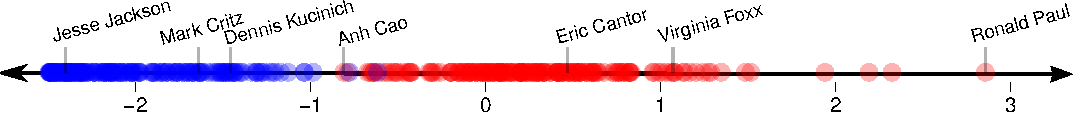
\includegraphics[width=0.95\textwidth]{chapter_predicting_votes_with_text/figures/3393_example_ideal_points_final.pdf}
  \caption{Example one-dimensional ideal points from the 111th House
  of Representatives.  Ideal points represent lawmakers' voting
  preferences. Democrats are blue and Republicans are red.}
  \label{fig:example_ideal_points}
\end{figure}

% dmb: i liked the section below about the utility model.  its
% interesting, but i propose we remove it or describe it in a
% paragraph somewhere else.  my reasoning is that its not essential to
% our story of ideal point-limitations-new model and, while elegant,
% its also complicated (i.e., introduces notation etc).  i want the
% reader to quickly understand ideal points and then start thinking
% about their limitations.  that said, i put a footnote about the
% utility model above.
% smg: got it.

% --- utility model begin ---



% \textbf{The Bayesian ideal point model.}
% The ideal point model is a generative model of choices (votes) and
% issues (bills).  Each legislator $u$ is associated with an
% \textit{ideal point} $X_u$ (see \myfig{ideal_points}), and each bill
% is associated with a \textit{discrimination} $B_d$ and
% \textit{difficulty} $A_d$.  The vote $v_{ud}$ is assumed drawn from the
% linear model
% \begin{equation}
%   \label{eq:ideal-point}
%   p(v_{ud} = \textrm{yea}) = \sigma(x_u b_d + a_d),
% \end{equation}
% where $\sigma(t) = \frac{\exp(t)}{1 + \exp(t)}$.  This is a logistic
% regression with random effects.\footnote{Some ideal point models use a
% probit model; we have found both approaches to ideal points to yield
% similar results}

% Notice the roles of the per-legislator and per-bill latent variables
% in \myeq{ideal-point}.  The difficulty parameter $a_d$ explains bills
% that all legislators will vote for or against, e.g., ``A bill to
% congratulate the winner of the World Series.''  For the remaining
% bills, i.e., those with some political division, the discrimination
% parameter $b_d$ and ideal point interact.  When estimated from roll
% call data, these latent variables capture the political leanings of
% the legislators and the political tone of the legislation.


\section{A model for predicting votes with the text of new bills}
%% Roll call data is essential for understanding government because it
%% represents atomic and concrete actions of its members.  But this data
%% is only one part of a richer record which includes bill texts,
%% speeches, press releases, public plans, and other items.  
 
In this section, we extend ideal point models to use the text of bills
to estimate a bill's polarity and popularity.  This gives a new way of
exploring and analyzing the government record and, further, gives a
useful predictor of government.  While traditional methods can only
fill in missing votes, we develop tools that can predict how lawmakers
will vote on a new bill. We will study the predictive accuracy of
votes on new bills, where we use a spatial voting model as a ``cold''
prediction mechanism.

% \begin{figure}[t]
%   \includegraphics[width=0.45\textwidth]
%   {chapter_predicting_votes_with_text/figures/134_senator_name_accuracy_by_ip_sample.pdf}
%   \caption{Sample Senator ideal points in the 111th Congress.  Ideal
%     points tend to separate the U.S. political parties: Democrat are blue,
%     and Republicans are red. A plot of all legislators is included in
%     the supplementary materials.}
% \label{fig:ideal_points}
% %\vspace{-22pt}
% \end{figure}

% DMB-2011: sean, above, can you make a more readable figure of ideal
% points?  For example, you can just show the senators or show a
% subset of the representatives.  Give specifics in the paragraph (and
% caption) about which legislature is illustrated.
% SMG: I've gone from Senators-only to a subset of ~20 Senators.
% DMB-2011: above, we need a citation for the psychometrics model.
% SMG: Done.

We will describe several models that connect the voting
patterns of lawmakers to the original text of bills.  One of these
models embeds the statistical assumptions of \textit{supervised topic
  modeling}~\citep{blei:2008} into the ideal point model, where the
locations of the bills are predicted from the latent topics in their
texts. This model---the ideal point topic model---can predict complete
votes on pending bills and provides a new way of exploring how
legislative language is correlated with political support.  The other
models predict inferred ideal points using different forms of
regression on phrase counts.

In the following sections, we review the details of ideal point
estimation and develop several models for predicting votes from
legislative text.  We derive an approximate posterior inference
algorithm for ideal point models based on variational methods and
analyze six Congresses (12 years) of legislative data from the United
States Congress.  Given a legislative history, these models can
accurately predict votes on future legislation.  One of these models,
the ideal point topic model, can help summarize and visualize the
political landscape of a government body based both on the voting
patterns of its members and the language of its issues.

\begin{figure}[t]
\center
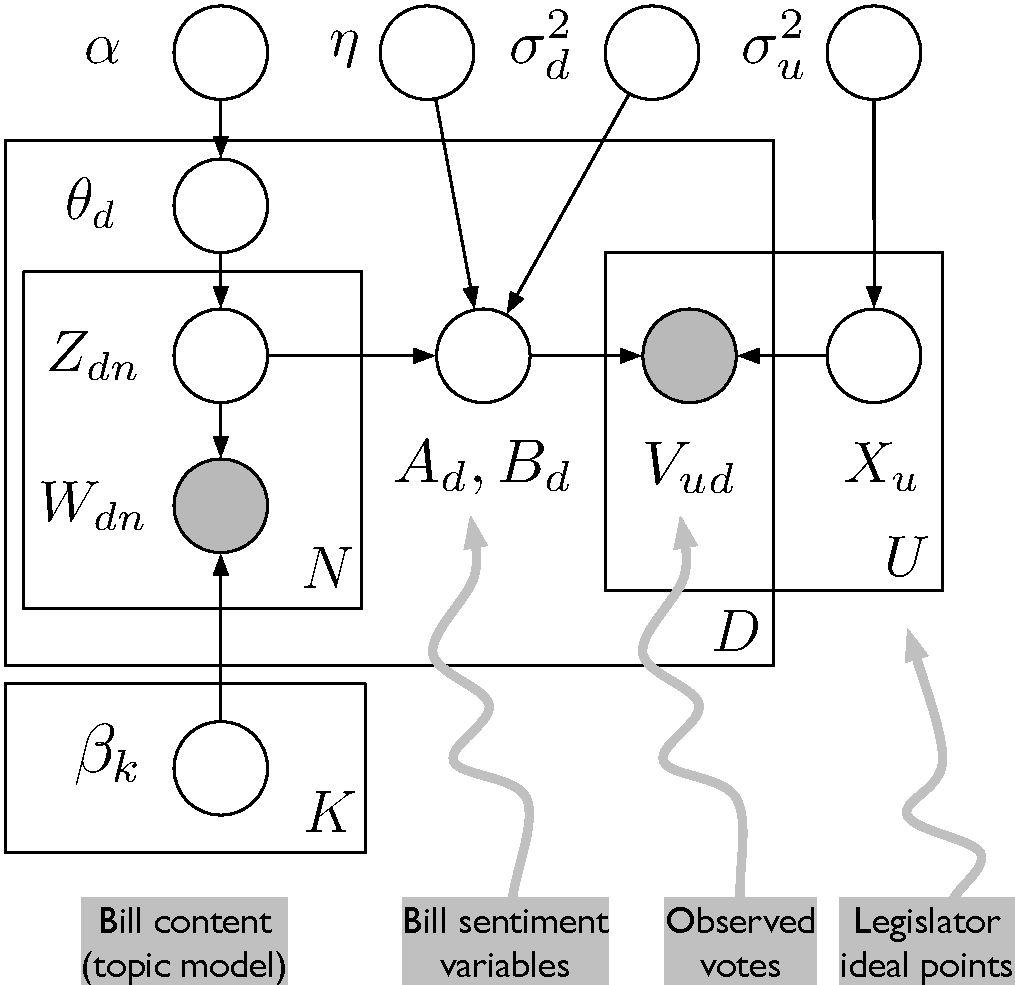
\includegraphics[width=0.5\textwidth]{chapter_predicting_votes_with_text/figures/ideal-point-topic-model.pdf}
\caption{The ideal point topic model.  Priors over the multinomials
$\theta_d$ and $\beta$ are both symmetric Dirichlet distributions.}
\label{fig:legis_gm}
\end{figure}

We now develop models relating the text of a bill to the variables
$a_d$ and $b_d$.  Associating text to bill variables has a predictive
advantage because new bills can be situated in the space of ideal
points.  It also has an interpretive advantage because language
becomes associated with political sentiment.

\textbf{Modeling ideal points with text regression.} We developed two
predictive ideal-point models which use text
regression~\citep{kogan:2009}.  For these, we first fit an ideal-point
model to a training set of bills and all lawmakers using the
variational algorithm described in \mysec{model}.  We then fit Lasso
regression\footnote{Implemented in the ``penalized'' package for R}
(\verb!LARS!)\footnote{implemented with the ``lars'' package for R}
and Ridge regression (\verb!L2!) to these bills' parameters $a_d, b_d$
using a vector of their $n$-gram\footnote{See \mysec{experiments} for
  details.}  counts $\bm w_{d}$ as covariates.

\textbf{Modeling ideal points with supervised topics.} The text
regression models link individual words or phrases to bill sentiment.
In this section, we connect textual \emph{themes} with bill sentiment.
We refer to this model as an ideal point topic model (IPTM).

To model themes, we use the assumptions of supervised Latent Dirichlet
Allocation (sLDA)~\citep{blei:2008}.  As in Latent Dirichlet Allocation
\citep{blei:2003}, each bill is represented as a mixture of latent
topics $\theta_d$, where each of $K$ topics $\beta_k$ is a multinomial
probability distribution over terms.  For the $n^{th}$ term of bill
$d$, we draw topic $z_{dn}$ from $\mbox{Mult}(\theta_d)$, and then
draw word $w_{dn}$ from the topic $\beta_{z_n}$.

% the Dirichlet prior for $\theta$ has parameter $\alpha$.

% DMB-2011: above, that point can be mentioned in the caption of the
% graphical model.  (that caption should summarize the rest of the
% notation too.  it's a good place for that.)

% DMB-2011: it also looks like we need to add the dirichlet prior on topics
% to the graphical model.

Like sLDA, the ideal point topic model further assumes each bill
$d$ is attached to a response variable.  In this case, the
response variable is the 2-component vector of bill variables $(a_d,
b_d)$.  The distribution of the response is a linear model whose
covariates are the empirical distribution of the topics $\bm z_d$ for the
bill,
\begin{align*}
  a_d &\sim& {\cal N}(\bm \eta_a^\top \bm \bar{z}_d, \sigma_d^2) \nonumber \\
  b_d &\sim& {\cal N}(\bm \eta_b^\top \bm \bar{z}_d, \sigma_d^2), \nonumber
\end{align*}
where $\bar{z}_d = (1/N) \sum_n z_{dn}$.  This setting is more complex
than the original sLDA model: the response variables are
\textit{hidden}---they are not observed directly, but are used
downstream in the voting model.

Finally, we add a Gaussian prior to $\bm \eta$.  The full model is
represented as a graphical model in \myfig{legis_gm}.

The only observed variables in the model are the bill texts and votes.
Our goal in fitting this model is to uncover the posterior
\begin{align}
  p(a_d, b_d, x_u, \bm \eta, \beta, z, \theta | \bm W, \bm V), \label{eq:posterior}
\end{align}
which can then be used in exploratory or predictive tasks.
Conditioned on these variables, our analysis proceeds with the
posterior distribution of the ideal points, polarities and
difficulties, topics, and coefficients. Computing the posterior exactly
is intractable, so we use variational inference to approximate it.  We
describe this in further detail in \mysec{inference}.

% DMB-2011: insert notation of the posterior here; just the LHS p(
% blah given blah).  it looks like something along the lines of the
% first paragraph of the inference section might do the trick.  then,
% in the inference section, just recall these tasks (and equations)
% and get right to why its difficult to actually do them.  (in fact,
% you can even mention that here too and forward point to the section
% on computation.)

% DMB-2011: outline the process of prediction above SMG: Prediction
% details were originally explained in the variational inference
% section.  I think it makes sense to leave them there, since we don't
% have variational parameters defined yet.
This posterior allows us to explore the connection between language
and political tone.  For example, the coefficients $\bm \eta$ are a
direct connection between bills' topics and the political tone of
these bills. Examples of this are provided in \mysec{experiments}.
The topics $\beta$, learned from both text and votes, provide a
lexical window into legislative issues.  The parameters $\bm \eta,
\beta$ together also allow us to predict votes using the text of new
bills; \mysec{inference} provides detail about this.

% DMB-2011: finish above too.  the idea is that the coefficients &
% topics together tell us how the model has associated language with
% discrimination or difficulty.  maybe forward point to some examples.

% The full likelihood of this model is given by
% \begin{eqnarray}
% \label{likelihood}
%   p(\bm W, \bm V, W, z, I, X, \theta, \bm \eta) = \nonumber \\
% & \hspace{-90pt} \prod_D  p(\theta_d | \alpha) \prod_N p(w_n | z_n, \beta)
%    p(z_n | \theta_d) \nonumber \\
% & \hspace{-90pt} \times \prod_D p(I_d | z_{d, 1:n}, \bm \eta) \times p(\bm \eta) \nonumber \\
% & \hspace{-90pt} \times \prod_U p(x_u) \prod_D p(v_{ud} | x_u, I_d). \nonumber \\
% \end{eqnarray}
% This likelihood is also represented in the graphical model in

%A. Ideal point model - we use logit, jackman, quinn use MCMC.  The
%results in \mysec{ideal} suggest that the results are very
%similar.

%  B. Supervised topics C. Full Likelihood function

\subsection*{Multimodal solutions and identification}
\label{sec:pv_identification}
Note that a fit of the ideal point model has multiple modes.  In one
mode, Democrats tend to have positive ideal points, while Republicans
are negative; in another, Republicans are positive, while Democrats
are negative.  To keep fits of the different models identifiable,
several researchers have applied nonzero priors over specific
lawmakers to encourage the model to prefer one of these modes
\citep{jackman:2001,clinton:2004,martin:2002}.

In the study in \mysec{experiments}, we anchor four lawmakers with
strong priors ($\sigma_d = 10^{-3}$) at ideal points $\pm 4$.  We
select two congresspersons from each chamber and two from each party:
Kennedy (S-Dem) and Waxman (H-Dem) are centered at +4 and Enzi (S-Rep)
and Donald Young (H-Rep) are centered at -4.\footnote{This value was
selected to be large yet not completely out of the ordinary.} We
selected these Senators for consistency with previous
work such as \cite{clinton:2004}.  We selected the Representatives because
they have held long offices in the House.  Without these sharp priors,
the model still discovers ideal points which cleanly separate
political parties but may converge on ``opposite'' modes in different
fits.  With the priors, we obtain consistent ideal points at the
expense of predictive performance.

\section*{Related work}

% Spatial voting models begin with a strong assumption about what
% causes individuals (often voting citizens) to vote as they
% do~\cite{enelow:1984}.
% % TODO(sgerrish): contrast these with other models of voting.

Ideal point models, a form of spatial voting model, have roots as far
back as the 1920s \citep{enelow:1984}. They are fit by both
frequentist~\citep{poole:1985,heckman:1996} and Bayesian
methods~\citep{jackman:2001,martin:2002,clinton:2004}, have been
embedded in a time series~\citep{martin:2002,wang:2010}, and have been
developed for higher dimensional political
spaces~\citep{jackman:2001,heckman:1996}.

% \nocite{jackman:2001}
\nocite{johnson:1999ch6}

Topic models have been applied to Senate speeches, such as to discern
``the substantive structure of the rhetorical [legislative] agenda''
\citep{quinn:2006}.  They have also been used with legislative speeches
to gauge lawmakers' sentiment toward legislation using roll-calls
\citep{thomas:2006}.  Modeling sentiment in text is more generally
discussed in the field of sentiment analysis; see \cite{pang:2008} for a review.

% DMB-2011: the above explanation is confusing.  how is a document
% drawn from a mixture of gaussians?  are there topics in their model?
% SMG: Clarified.

The ideal point topic model relates closely to user-recommendation
models based on matrix factorization~\citep{salakhutdinov:2008a}.
Matrix factorization methods for recommendation are akin to
large-scale spatial behavior models (though usually with no
``difficulty'' term, which acts as an intercept).  Many of these
matrix factorization models for user recommendation do not provide a
method of predicting one user's item preference without other users'
preferences on the same item.

Two works stand out as closely related to this work.  One of these is
fLDA, which models binary or continuous ratings with user affinity to
topics \citep{agarwal:2010}.  Another is \cite{wang:2010}, who
describe a similar application by combining topic models and matrix
completion.  Their work also draws on ideal point models, models
transitions over time, and is designed to learn the dimensionality of
the latent factors.  Under the generative assumptions of their model,
bills and matrix cells (e.g., votes) are conditioned on a shared
mixture; in our model, votes are conditioned on words' topics.

% \cite{poole:1985} Present a spatial model for analyzing
%roll-calls.

% - poole and rosenthol K. T. Poole and H. Rosenthal.  ``A Spatial
% Model for Legislative Roll Call Analysis.''  American Journal of
% Political Science, Vol 29 (1985a), pp. 356-384 - present NOMINATE.
% Is a \cite{heckman:1996} Present a linear probability model known as
% NOMINATE.  Application to roll-call analysis.


% \cite{johnson:1999ch6} Provides discussion of Bayesian inference and
% model checking for item-response models.  Johnson (ch. 6) notes
% Early analysis of item response models are found in Swaminathan and
% Gifford (1982, 1985) and Tsutakawa and Lin (1986).  Patz and Junker
% (1997) demonstrate Metropolis within Gibbs simulation for Bayesian
% Item Response models with Logistic link.

% heckman: probabilistic models for inferring votes - linear
% probability model of preferences motivated by rational choice theory
% for economics - uses an ideal point, or ``bliss point'' -
% justification: taylor approximation of utility - factor-analytic
% model (according to jackman) - produces consistent estimates - find
% at least 6 statistically significant dimensions - model goods:
% computational simplicity, ability to rigorously estimate dim.

% - enelow and hinich: euclidean spacial voting model (1984) ``The
% Spatial Theory of Voting: an Introduction'' 1984 J. Enelow and
% M. Hinich Cambridge University Press.  New York.

% K. T. Poole and H. Rosenthal.  ``Analysis of Congressional Coalition
% Patterns: A Unidimensionaal Spatial Model.''  American Journal of
% Political Science, Vol 29 (1985a), pp. 356-384 Spatial Models of
% Legislative Voting, Keith T. Poole.  - in 1997 present D-NOMINATE.
% - nonlinear probability model - assume logistic model of

% - Rabinowitz and McDonald: directed preference model (1989)

% - gorman

%    W-nominate is normal-logit
%    NOMINATE
%     - max-likelihood estimation.  does not produce consistent estimates.


%  B. Ideal point models
%    - jackman, clinton take Bayesian approach, to take advantage of
%    the MCMC sampling machinery for inference, and to make inferences and
%    substantive hypotheses about ideal points.

%    - in addition, Jackman notes that the methodology can provide a coherent framework of hypothesis testing \cite{gelman:1996}
%    - compare this approach with

%%% Local Variables:
%%% mode: latex
%%% TeX-master: "icml2011"
%%% End:

\section*{Posterior estimation for the ideal point topic model}
\label{sec:inference}
Computing the posterior in \myeq{posterior} is intractable.  Posterior
inference for traditional Bayesian ideal point models is traditionally
implemented with MCMC methods such as Gibbs sampling
\citep{johnson:1999ch6,jackman:2001,martin:2002,clinton:2004}.
However, in the ideal point topic model, fast Gibbs samplers are
unavailable because the conditionals needed are not analytically
computable; an MCMC strategy would require a more complicated sampling
scheme. We therefore use an alternative algorithm -- which can be applied
to both the standard ideal point model and the ideal point topic model
-- which uses variational methods \citep{jordan:1999}.

Recall from Chapters 2 and 3 that variational inference requires
specification of a variational distribution which will serve as a
proxy for the true posterior distribution.
% dmb: make it clear that we use a fully-factorized variational
% distribution.
% smg: added a note below.  We use a fully-factorized variational
Word assignments $z_{dn}$ and topic proportions are governed by
multinomial parameters $\phi_d$ and Dirichlet parameters $\gamma_d$,
as in LDA~\citep{blei:2003}.  The variational distribution for
lawmakers' ideal points $x_u$; bills' parameters $a_d, b_d$; and
coefficients $\bm \eta$ are Gaussian with respective means $\tau_u$,
${\tilde a}_d$, ${\tilde b}$, $\ev$ and variances $\sigma_\tau^2$,
$\sigma_{\tilde a}^2$, $\sigma_{\tilde b}^2$, and $\sigma_\eta^2$. The
variational distribution is
\begin{align}
\label{eq:var_post}
q(\tau, & \sigma_\tau, {\tilde a}, \sigma_{\tilde a}, \phi, \theta) =
  \prod_u q(x_u | \tau_u, \sigma_\tau^2 ) \prod_D q(a_d, b_d |
{\tilde a}_d, \sigma_{\tilde a}^2 )
  \prod_D q(\theta_d | \gamma_d)
  \prod_{N_d} p(z_n | \phi_n) q(\bm \eta | \ev, \sigma_{\ev}).
\end{align}

Inference proceeds by minimizing the KL between the variational
posterior (\myeq{var_post}) and the true posterior (\myeq{posterior}),
which is equivalent to maximizing a lower bound on the marginal
probability of the observations.  Coordinate ascent only works for
some of the random variables, but we must use gradient ascent on $a_d,
b_d,$ and $x_u$.  We give further details of the variational inference
algorithm in \myapp{iptm_app_variational_inference}.

\textbf{Prediction} After they are fit to lawmakers' votes and bill
text, the variational parameters $\tau$, $\ev$, and $\beta$ can be
used to estimate the vote of each lawmaker on a \emph{new} bill $d$
using its text.  To predict whether lawmaker $u$ votes \verb!yea! on
$d$, the per-word parameters $\phi_n$ of $d$ are estimated using the
topics $\beta$. Once $\phi$ has been estimated, the probability of a
\verb!yea! vote is given by $p(v_{ud} = \verb!yea!)  = \sigma(\tau_u
(\bar{\phi_d} \ev_b) + \bar{\phi_d} \ev_a)$
\footnote{The estimate $\expectq{\sigma(x_u (\bar{z_d} \eta_b) +
    \bar{z_d} \eta_a)}$ can be more theoretically justified, but
  results from the two estimates are (in practice) identical.}, where
$\bar{\phi_d}$ is $\frac{1}{N_d} \sum_{N_d} \phi_n$.  In practice, we
fit $\ev$ with no regularization after the model has converged.  This
gives slightly better results which are more robust to parameter
selection.

\section{An empirical analysis}

\begin{figure}
\label{fig:log_likelihood}
\begin{center}
  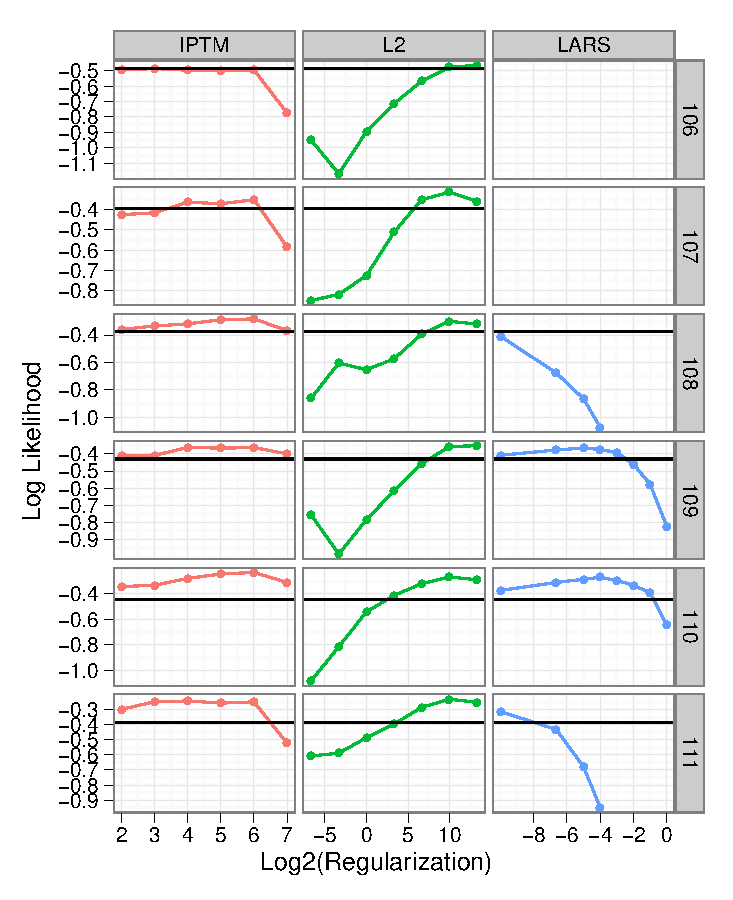
\includegraphics[width=0.9\textwidth]
{chapter_predicting_votes_with_text/figures/138_log_likelihood_by_session_topics.pdf}
\end{center}
\vspace{-6pt}
\caption{Vote log likelihood on heldout votes. Models are shown
  by color for different regularizations (x axis), for Congresses 106
  to 111.  For LARS and L2, the regularization is the complexity
  parameter; for the ITPM, the regularization is the the number of
  topics.  The \emph{yea} baseline is the horizontal black line. LARS
  is below the fold for 106-107.  The ideal point topic model performs
  with less variance across its regularization parameter. }
\vspace{-3pt}
\end{figure}
\subsection*{Analyzing the U.S. House and Senate}
\label{sec:experiments}

We studied the performance of these models on 12 years of data from
the United States House of Representatives and Senate.  We first
demonstrate how the ideal point topic model can be used to explore
legislative data; then we evaluate the models' generalization
performance in predicting votes from bill texts.

We collected roll-call votes for Congressional sessions 106 through
111 (January 1997 to January 2011).  We used votes about bills and
resolutions, and only votes regarding the legislation as a whole
(as opposed to, e.g., amendments of the legislation). We downloaded
the data from Govtrack, an independent Website which provides
comprehensive legislative information to the public.  Our
collection contains 4,447 bills, 1,269 unique lawmakers, and
1,837,033 \verb!yea! or \verb!Nay! roll-call votes.

To select the vocabulary, we lemmatized (i.e., normalized the forms
of) words in the bills with Treetagger~\citep{treetagger}.  Then we
retained a vocabulary of statistically significant $n$-grams ($1 \le n
\le 5$) using likelihood ratios.  These $n$-grams were treated as
terms.\footnote{When one $n$-gram subsumes another, we chose to
  observe the longer of the two} We removed $n$-grams occurring in
fewer than 0.2\% of all bills and more than 15\% of bills.  We also
removed an $n$-gram if it accounted for more than 0.2\% of all tokens
or fewer than than 0.001\% of all tokens.  After this process, our
vocabulary contained 4,743 unique $n$-grams.

We used the anchor lawmakers described in \mysec{model}.  We ran
variational inference until the change in increase in the objective
function was less than 0.01\%.

\subsection*{Exploring topics and bills}

In this section, we examine a fit of the ideal point topic model for
all the bills and votes of a session.  This demonstrates the model's
use as an exploratory tool of political data.  For this analysis, we
used dispersion $\sigma_d = \sigma_u = 1.0$ and 64 topics.  We focus
on the $111^{th}$ session (January 2009 to January 2011).

\textbf{Exploring topics with $\ev$.} As noted in \mysec{model}, the
coefficients $\ev$ relate each topic's weight in a bill with the
bill's difficulty and polarity parameters. \myfig{topics} shows
some example topics and their corresponding coefficients $\ev$.  Below
we describe some of these topics in more detail and connect them to
the data.

\begin{figure}
  \center
  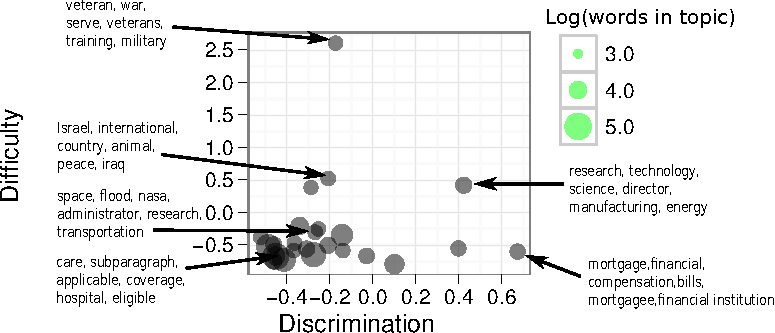
\includegraphics[width=0.9\textwidth]{chapter_predicting_votes_with_text/figures/134_64_topic_plot.pdf}
  \caption{Topics can be visualized in the same latent political space
    as lawmakers and bills.  This plot shows selected topics by
    coefficients $\ev$, for a 64-topic model ($\ev$s are normalized by
    mean and variance).  Two topics (\emph{people, month, recognize, ...}
    and \emph{clause, motion, chair, ...}) with difficulty 4.68 and
    polarity 7.4 (respectively) are not shown.}
  \label{fig:topics}
\end{figure}

One popular topic in the 111th Congress focused on national
recognition: \emph{people, month, recognize, history, week, woman}.
In contrast, the \emph{least}-supported topic was more procedural,
frequently appearing in bills under consideration or with many
amendments (\emph{clause, motion, chair, print, offer, read}).  In
this case, such legislation is sometimes summarily rejected before
further consideration; the language of amendments is a signal that
legislation is contentious.

While these topics often explained overwhelming support or rejection
of legislation, much legislation was considerably more partisan.

\textbf{Health Care.}  One contentious topic was about
% parameters: Discrimination 0.122, Difficulty 4.75
qualification for public health care: \emph{care, subparagraph,
applicable, coverage, hospital, eligible}.  This topic was among the
most-Democratic 10\% of topics, in large part because it helped to
explain the \emph{Patient Protection and Affordable Care Act},
i.e. the ``Health Care Bill'' of 2009.  Although this 906-page bill
was barely passed: of the 311 Democrats voting on
it, 276 voted in favor; of the 217 Republicans voting on it, none
voted in favor.  The model was moderately accurate on this bill: it
correctly predicted 93.8\% of votes.  The two other topics highly
expressed in this bill were about different aspects of public health,
including one about government health options (medicare and social
security) and one about health insurance coverage; both were slightly
Democratic.

\textbf{NASA Authorization.}
Another contentious topic was about spaceflight: \emph{space, flood,
NASA, administrator, research, transportation}.
This topic was expressed in one of the most-poorly predicted bills of
the $111^{th}$ Congress.  This bill, the \emph{NASA Authorization Act
of 2010}, was a "compromise between the Obama administration, which
wants... a commercial space industry in which private companies would
transport astronauts, and House lawmakers, who wanted... one
government-owned rocket" \citep{herszenhorn:2010}.  In the house vote
(a Senate record was not kept), of 249 Democrats voting on the bill,
185 voted in favor; of the 173 Republicans, 119 voted in favor.
Because this bill had mixed but nonpartisan support, the model could
not represent it well, with only 72\% of votes correctly predicted.

\subsection*{Checking the ideal points}
We can also use the in-sample fit to assess the quality of the ideal
points of the lawmakers.  In classical ideal point modeling, this is
done via in-sample accuracy: How well does the model explain the
observed votes?

The average per-lawmaker accuracy in the in-sample fit was 96\%
(only 10\% of lawmakers had accuracy lower than 90\%).  As expected,
accuracy increases with more votes ($\rho=0.51$).  Among lawmakers
with over 100 votes, only two stand out. Donald Young (713 votes;
accuracy 0.83) had a pre-defined ideal point (see \mysec{model}). Ron
Paul, a Republican in the $111^{th}$ Congress, was also poorly
predicted (761 votes; accuracy 0.84).  Paul is known for his
Libertarian beliefs, even having run for President for the Libertarian
party in 1988.

The poor prediction of Paul points to a limitation of the
1-dimensional ideal-point model, which can only capture the two main
parties, instead of a limitation of the supervised prediction: fitting
votes to the classical ideal point model (ignoring bill text), Paul's
in-sample accuracy was consistently poor across sessions.  We will
address this limitation in the next chapter by incorporating a bill's
issues in the prediction task.

\subsection*{Predicting votes from text}

\textbf{Prediction on heldout bills.}  We measured predictive accuracy
and log likelihood for these models under a variety of regularization
settings (\verb!LARS! is parameterized by $0 < f \le 1$, \verb!L2! is
parameterized by $\Lambda \ge 0$, and \verb!IPTM! is parameterized by
topics $K$).

We also devised two baselines for comparison with the three models
described so far.  The first of these provides a lower bound: assume
all votes are \verb!yea!.  Because the majority (85\%) of votes in our
corpus were \verb!yea! votes, this presents a more reasonable overall
baseline than random guessing (at 50\%).  We call this model the
\verb!yea!  model.  The second baseline fit a logistic regression
trained for members of each party (with a separate one for mixed or
independent lawmakers), with terms as covariates.  This baseline
(implemented with the R \verb!glm! library) used too much memory to
use more than 800 terms and therefore led to results worse than the
\verb!yea!  baseline.  We believe that a better baseline could be used.

For each 2-year period (called a Congress), the bills were partitioned
into 6 folds.  For each model, we iteratively (1) remove a fold, (2)
fit the model to the remaining folds (by Congress), and (3) form
predictions on the bills in the removed fold.  Across folds, we thus
obtain a complete data set of held-out votes.

Across all sessions, the \verb!yea! baseline predicts votes correctly
85\% of the time.  The ideal point topic model is better, correctly
predicting 89\% of votes with 64 topics (this means that 62,000 more
votes are correctly predicted).  Overall performance for \verb!L2! was
best for $\Lambda=1000$ (90\%), and \verb!LARS! was best at $f=0.01$
(82\%).  While the ideal point topic model had lower accuracy than
\verb!L2!, its log-likelihood was nearly the same.  These results are
summarized in \myfig{log_likelihood}, and further details are in
\myapp{iptm_app_experimental_results}.

\textbf{Sequential prediction.}  Our final study examined the
performance of these models on predicting future votes from past
votes.  To do this, we fit a 64-topic \verb!IPTM! and \verb!L2!
predictive models on the first $3, 6, 9, \ldots, 21$ months of a
Congress.\footnote{A bug prevented LARS from completing in most runs of
this setting}  We then tested these each of these fits on the
following three months of unseen votes.  The ideal-point topic model
correctly predicted $87.0\%$ of votes, and \verb!L2!  correctly
predicted 88.1\% of votes; their log-likelihood was identical.

With these models, one could predict 31,000 to 55,000 votes
above the baseline, \emph{based only on the text of the bills}.  The
simpler of the two models, \verb!L2!, performs better at prediction.

\section{Conclusions and limitations of these models}

We have developed several models associating the text of legislation
to lawmakers' voting patterns.  These models provide a way of
exploring large collections of legislative data and predicting the
votes of new bills.  The text-regression models and the ideal point
topic model have incorporated bill texts into the simplest kind of
ideal point model of roll call data. 

Though we were motivated by (and focused on) political science data,
we note that these models are among several (e.g.,
\cite{agarwal:2010}) that can be applied in a variety of collaborative
filtering settings.  They provide a way to model a collection of users
and their decisions about collections of textual items.

One of the central advantages of latent-variable models is their
modularity.  Because we have modeled the text of legislation as a
vector of topics (or a vector of word counts), it is straightforward
to incorporate other elements of the legislative process, such as
speech transcripts \citep{quinn:2006,thomas:2006} or bill sponsor, into
this model's supervision.  This could improve both the predictive
power and exploratory capabilities of the ideal point topic model.
The modularity of latent-variable models allows us to swap in modeling
assumptions for each of these types of data.
 
However, even optimal features for prediction would be limited by the
power of the downstream model for lawmakers' votes on bills.  Here we
have studied multiple topics with a one-dimensional political space.
As noted in \mysec{experiments}, this is a predictive bottleneck. (The
``true'' number of dimensions is debatable---\cite{heckman:1996}
argued that there are at least 6 statistically significant dimensions
in roll-call data, while \cite{jackman:2001} barely found more than
one.)  One solution is to increase the dimension of the lawmaker and
bill variables or use a mixture model as in \citet{wang:2010}, which
can increase the strength of the model at the expense of
interpretability.

An alternative solution is to model individual lawmakers' affinities
to issues, using ideas explored by \cite{agarwal:2010} and
\cite{wang:2011} for matching users with text content.  We will use
these ideas in the following chapter, where we explicitly model
lawmakers' positions on a variety of issues.  This will allow us to
represent lawmakers' votes better than an ideal point model while
providing an interpretable window into individual lawmakers' voting
behavior.
